%% Qualitative comparison against the baselines on the full pipeline benchmark (two columns).
%% Graphic: figures/full_pipeline_comparison.png
%% Six labeled row blocks, top to bottom:
%%   (a) reference touch   (b) tactile normal quilting   (c) implicit neural representation
%%   (d) ours, coarse transfer   (e) ours, refined   (f) ground truth
%% Columns are frames 7, 12, 17, 22, 27, 32, 37 and 42 of the 50-frame press.
%% Row and column labels are baked into the image.
\begin{figure*}[t]
  \centering
  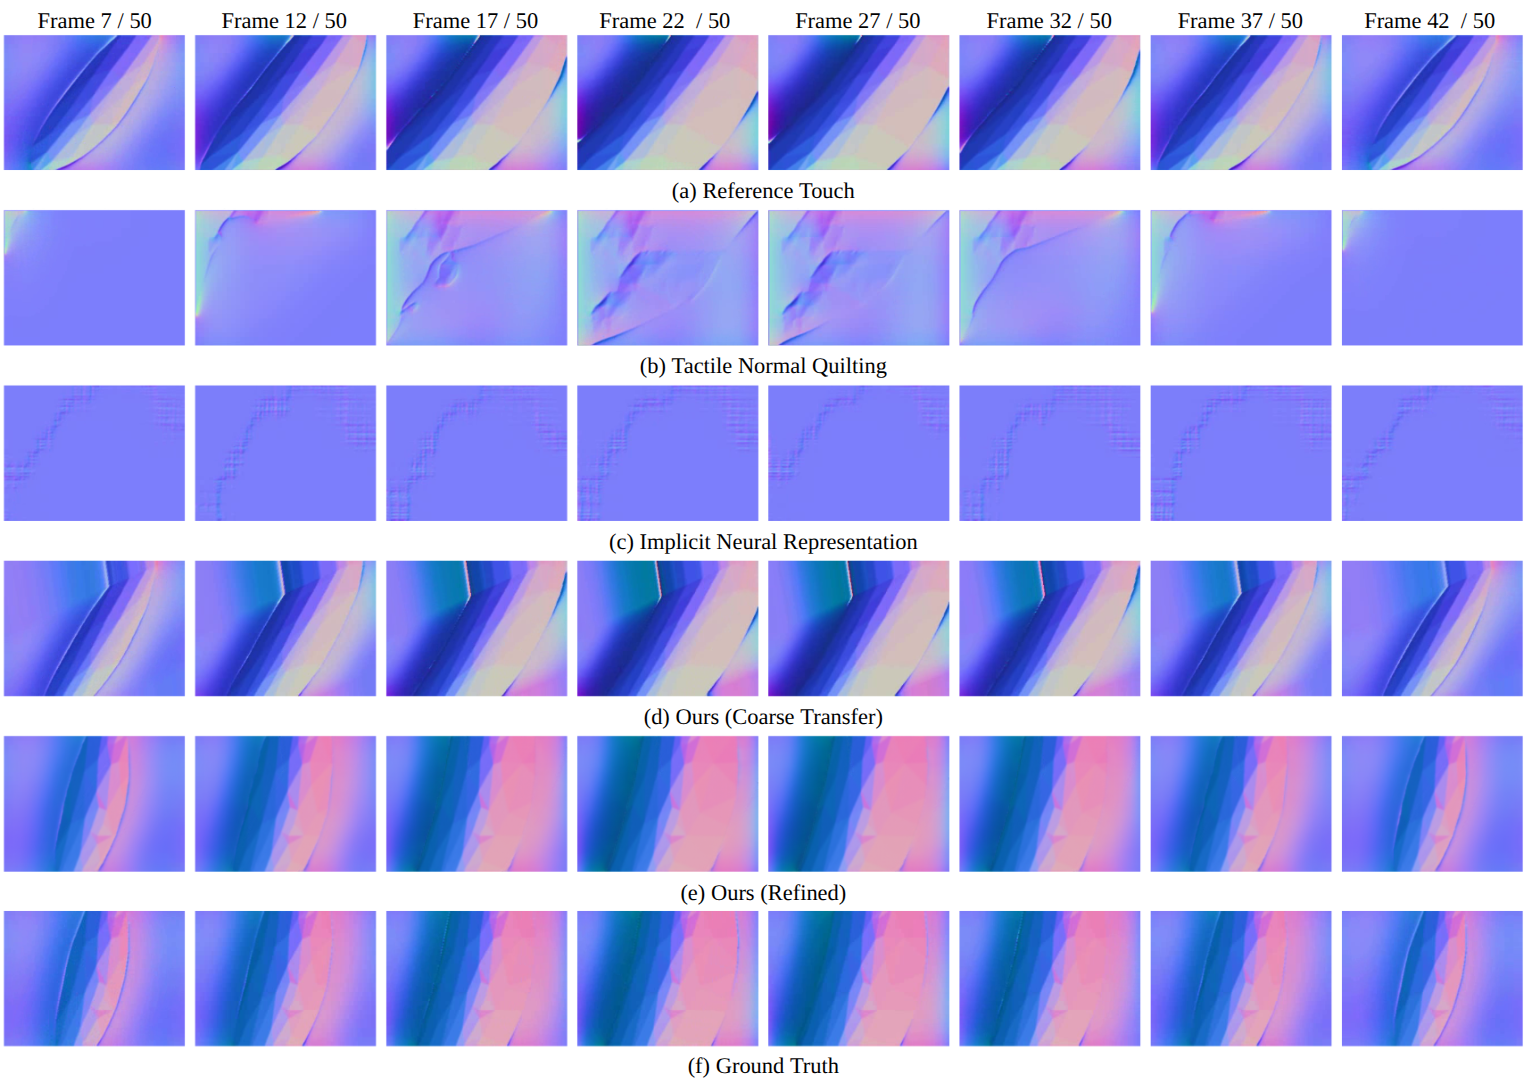
\includegraphics[width=\linewidth]{figures/full_pipeline_comparison.png}
  \caption{\textbf{Comparison against baselines on the full pipeline benchmark.} Each block of
    rows is one method and each column is a frame of the tactile normal video, sampled evenly
    across the 50-frame press. \emph{(a)} The reference touch that the prediction is transferred
    from, retrieved automatically from the object's other touches. \emph{(b)} Tactile normal
    quilting, which synthesizes a plausible texture but does not agree with the surface under the
    sensor. \emph{(c)} The implicit neural representation, which reproduces little beyond a faint
    outline of the contact and shows grid artifacts from its coordinate encoding. \emph{(d)} Our
    coarse transfer, which places the contact correctly but carries the reference press's own gel
    dynamics and warp artifacts. \emph{(e)} Our refined prediction, and \emph{(f)} the ground
    truth at the query location. Our refined result accurately tracks how the contact grows and recedes
    over the press while matching the geometry the sensor actually meets.}
  \label{fig:full_pipeline}
\end{figure*}
